\section{Risk factors of stablecoins}\label{sec:risk_factors}

A holder of a fiat-backed stablecoin carries, however briefly, a private-issuer liability convertible into the fiat unit of account at par on a best-effort basis. That promise can fail in two ways, and the two failures are economically distinct. The issuer may not hold enough liquid reserves of sufficient credit quality to honour redemption at par, in which case the holder bears a \emph{counterparty} loss. Or the market for converting the liability outside the issuer's primary venue may be too thin, so the realised conversion price falls below par when demand to convert is high, in which case the holder bears a \emph{depeg} loss. The sender of a stablecoin payment therefore bears a risk premium with two components. This section sets out each in turn: a counterparty component, which is an issuer-level credit exposure we read from market proxies, and a depeg component, which is a coordination outcome we price with a global game, formalised in Section~\ref{sec:model}.

\subsection{Counterparty credit risk}\label{sub:counterparty}

The counterparty component is the expected loss from issuer default. A holder of one unit faces a default hazard $h$ over the holding horizon and, conditional on default, a loss given default $\xi$ equal to the shortfall of recoverable reserve value against par. The expected per-unit loss is $h\cdot\xi$. This is a standard credit exposure on a short-dated claim against a private issuer; it does not depend on the redemption behaviour of other holders, and we price it in reduced form from observable market proxies for the issuer's reserve quality and default likelihood rather than from the coordination model of the next subsection.

The proxies that discipline $h$ and $\xi$ exist for both issuers, and they point in different directions. USDC is backed exclusively by short-dated US Treasuries and cash deposits at globally systemic banks, with monthly attestations and daily disclosure of holdings since 2022; its reserve is transparent and its loss given default correspondingly low. USDT holds a heterogeneous mix of US Treasuries, secured loans, and historically commercial paper, with attestations produced by BDO that lack the granularity of a full audit, and a residual uncertainty compounded by its enforcement record (the 2021 New York Attorney General and CFTC settlements). The implication for the model is direct: USDC's loss-given-default parameter $\xi$ is structurally lower than USDT's, and USDT's hazard $h$ is structurally higher. On the counterparty dimension the two coins are different animals, and a single number applied to both would misprice one of them.

We anchor the two parameters at values consistent with these market signals rather than estimating them inside the coordination model. For USDC we set a one-year issuer hazard $h=0.01$ and a loss given default $\xi=0.20$: a hazard of the order of a high-grade short-dated claim, matching the regulated cash-and-Treasuries reserve, and a low loss given default reflecting the liquidity and seniority of those reserves. For USDT we set $h=0.02$ and $\xi=0.30$, a roughly one-notch-lower credit standing and a higher loss given default consistent with the heterogeneous reserve, the attestation-only disclosure, and the enforcement record. The product $h\,\xi$ is the \emph{expected}, not the stressed, counterparty loss: the ten-cent intraday discount USDC reached during the March 2023 banking weekend is a depeg, priced by the global game below, not a realised default, and the resulting counterparty component of twenty basis points is the small ex-ante hazard rather than that ex-post discount. Section~\ref{sec:empirical_comparison} and Appendix~\ref{app:sensitivity} report how the premium moves as $(h,\xi)$ range over their plausible values.

\subsection{Depeg risk and the global game}\label{sub:depeg}\label{sec:global_game_policy}

The depeg component is not a credit exposure but a coordination outcome. Even a fully solvent issuer can deliver below par when many holders convert at once: primary redemption pays par only up to liquid reserves $R$, unmet demand spills into a secondary market of finite, stress-contracting depth, and the realised conversion price falls. A holder who anticipates others converting at the same time anticipates a worse price, so the decision is strategic, not individual. We model it as a global game in the spirit of \citet{morris_shin_1998}, adapted to the dual-channel exit through the issuer's primary redemption and a secondary market with depth-dependent price impact that distinguishes a stablecoin from a deposit. Figure~\ref{fig:global_game} shows the coordination structure.

\begin{figure}[p]
\centering
\includegraphics[width=\textwidth]{figures/fig_morris_shin_clock_preview.pdf}
\caption{Coordination structure of the stablecoin redemption problem. The depeg is a coordination outcome: conversions exhaust the issuer's primary redemption and depress the secondary price, a self-fulfilling run. Each holder observes the same fundamental $\theta$ with an idiosyncratic noisy signal $s_i$, picks a redemption threshold $s^{*}$ given the aggregate run she expects from the rest, while the aggregate run itself is determined by the threshold every holder uses. Equilibrium is the unique fixed point $s^{*}$ such that $B(s^{*}) = s^{*}$. The formal derivation is in Section~\ref{sec:model}.}\label{fig:global_game}
\end{figure}

A global game is the natural model rather than a stylised analogy because the secondary conversion price is not a market prior but an equilibrium object: the value of converting depends on how many others convert, through the price impact their conversions create, so the redemption decision is a coordination problem with a unique threshold equilibrium. That uniqueness is what lets the calibration map an observed price path into a single premium. The depth and convexity of the secondary market are themselves structural primitives that differ across issuers: USDT is the most liquid stablecoin globally, with primary venue Binance and per-side depth above USD 100 million, so its price-impact scale and depth erosion are structurally smaller, whereas USDC's venue (Coinbase) is shallower and its permissionless redemption more atomistic, raising its signal noise.

The two largest historical depeg episodes show the phenomenon directly, and they are the episodes we calibrate to. Figure~\ref{fig:svb_onchain} plots USDC during the March 2023 Silicon Valley Bank failure: the secondary price fell to about 0.90, the shaded below-par area being the holder's loss, as Circle's primary redemption was constrained by the banking closure; the on-chain redemptions that clear at par surged only once the federal backstop restored the peg. Figure~\ref{fig:terra_onchain} is the mirror image, USDT during the May 2022 Terra collapse: primary redemption stayed open, about USD 8 billion was redeemed at par, and the depeg was a brief dip to 0.975. The depth of a depeg thus turns on whether primary redemption remains available, the mechanism the global game formalises and Section~\ref{sec:identification} tests.

\begin{figure}[H]
\centering
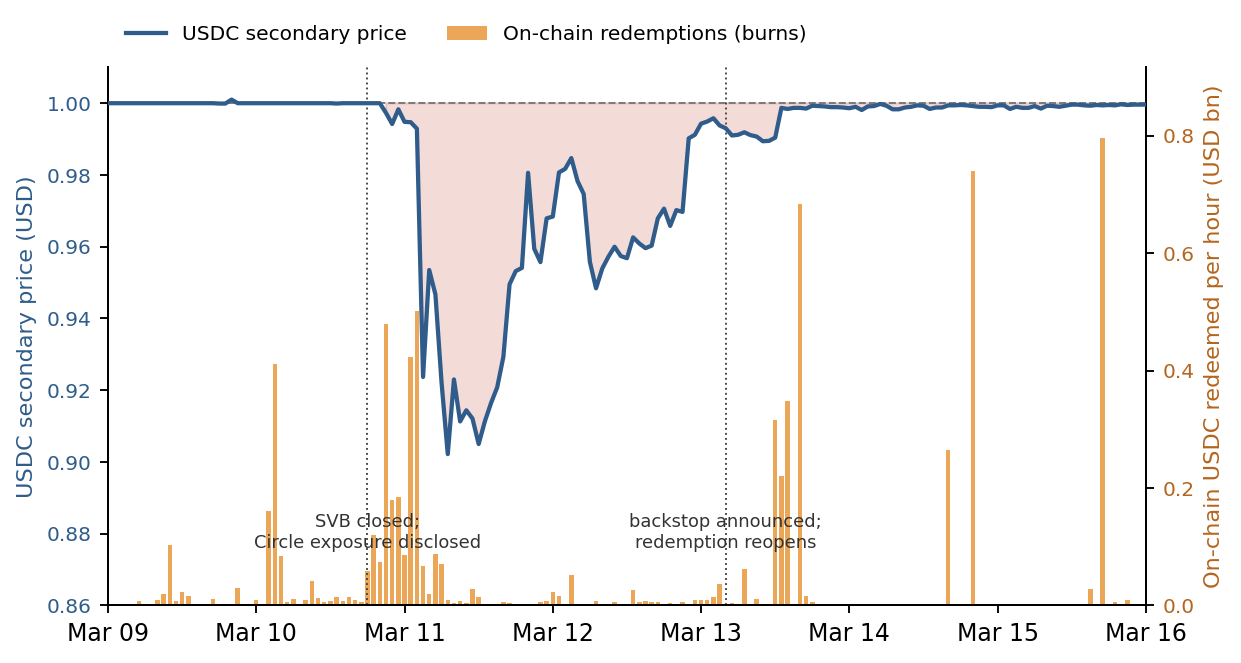
\includegraphics[width=\textwidth]{figures/fig_svb_onchain.pdf}
\caption{USDC during the March 2023 Silicon Valley Bank episode. Left axis: the hourly USDC secondary price, with the shaded area marking the below-par depeg. Right axis: hourly on-chain redemptions (token burns), from Etherscan. The depeg opens while primary redemption is constrained by the banking closure over 11--12 March; the at-par on-chain redemptions are largest only after the federal backstop restores the peg on 13 March. The holder's cost is the secondary discount borne while par redemption is unavailable, not the orderly redemptions that follow.}\label{fig:svb_onchain}
\end{figure}

\begin{figure}[H]
\centering
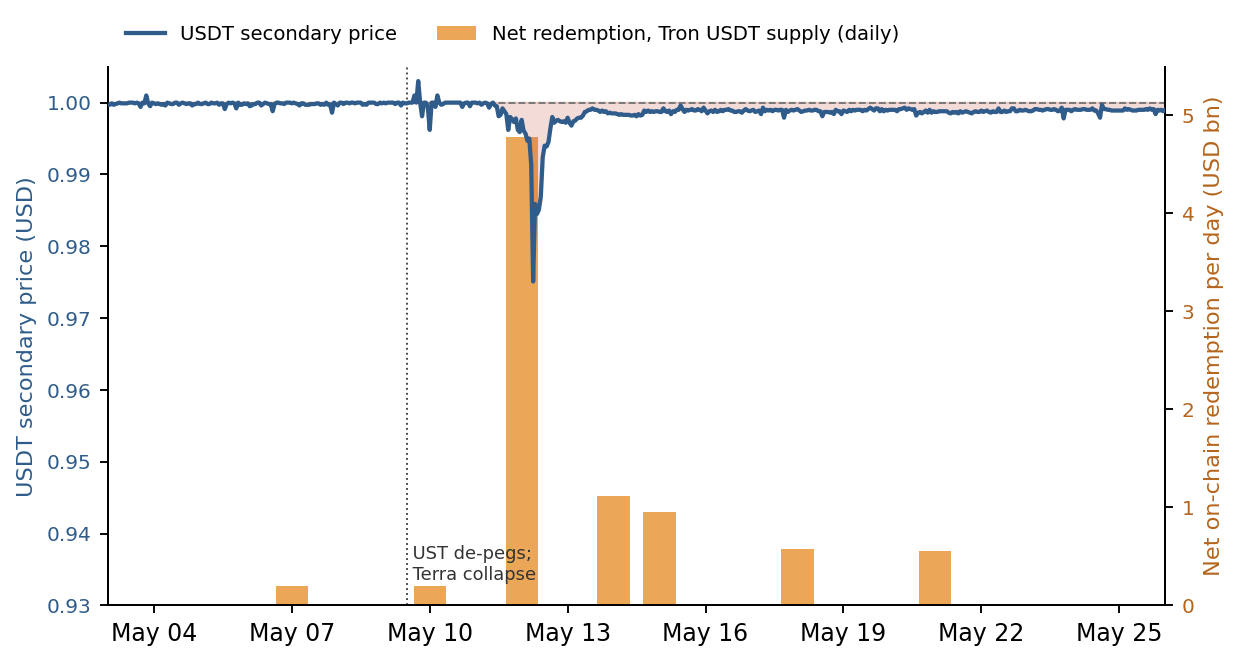
\includegraphics[width=\textwidth]{figures/fig_terra_onchain.pdf}
\caption{USDT during the May 2022 Terra episode. Left axis: the hourly USDT secondary price, with the below-par depeg shaded. Right axis: daily net redemption, measured as the contraction of USDT's Tron circulating supply. Primary redemption stayed open, about USD 8 billion was redeemed at par, and the depeg was a brief dip to 0.975, the mirror image of the USDC episode in Figure~\ref{fig:svb_onchain}.}\label{fig:terra_onchain}
\end{figure}

Section~\ref{sec:model} sets out the model formally, and Section~\ref{sub:what_it_delivers} combines the two risks into the premium the holder bears.
